\section{Results}

\subsection{Ois River}\label{sec:ois_river}       %% Ois river




\subsubsection{Length-frequency distribution}\label{sec:ois_fish_lf}

This distribution of salmonid length in the investigated area of the Ois ranged from 45mm to 433mm.
72\% of the total catch had a length of less than 120mm, which is the threshold for young-of-the-year (YOY) fish.
Distribution of adult fish can be see in~\cref{fig:avg_length}.
Fish length among the mesohabitats trends toward the largest fish in pools, decreasing in size to runs and then riffles containing the smallest fish.
The median length of brown trout was similar in the riffle and run sections.

The Rothschild section of the river had similar length brown trout populations when compared to the Hinterleiten.
The rainbow trout populations in the Rothschild were significantly larger than that of the Hinterleiten in all three mesohabitats.
Additionally, the rainbow trout populations in all sampled areas were larger than the brown trout populations.

\begin{figure}[!htb]                              %% Average length of 1+ years
	\center
	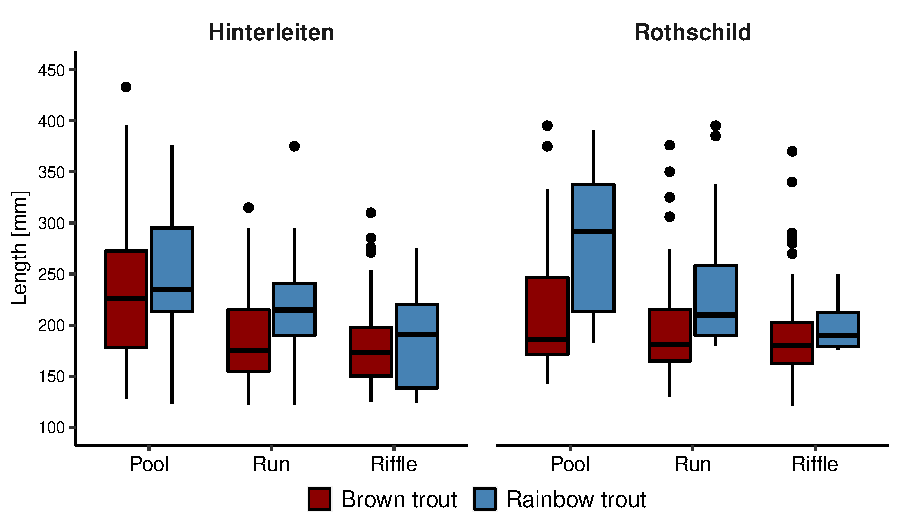
\includegraphics[width=.7\textwidth]{images/avg_length.pdf}                %% Width, Image file COLOR
	\caption{Boxplots displaying length of adult fish in investigated mesohabitats.}      %% Figure Caption
	\label{fig:avg_length}                                                       %% Figure label key
\end{figure}


\paragraph{Brown trout (\textit{Salmo trutta})}\label{sec:ois_bt_lf}

A very healthy brown trout population can be seen in the length-frequency chart of the combined sample areas~(\cref{fig:brown_single}).
A total of 1866 brown trout were caught in 9 sample sites.
Fish of less than 120mm in length represent the YOY, while the 1+ age class (\textgreater120mm) and 2+ age class (\textgreater220mm) are clearly visible along with several individuals larger than 300mm.
YOY fish account for the majority of the catch at 74\%, indicating successful spawning.

\begin{figure}[!htb]                              %% Brown in Ois
	\center
	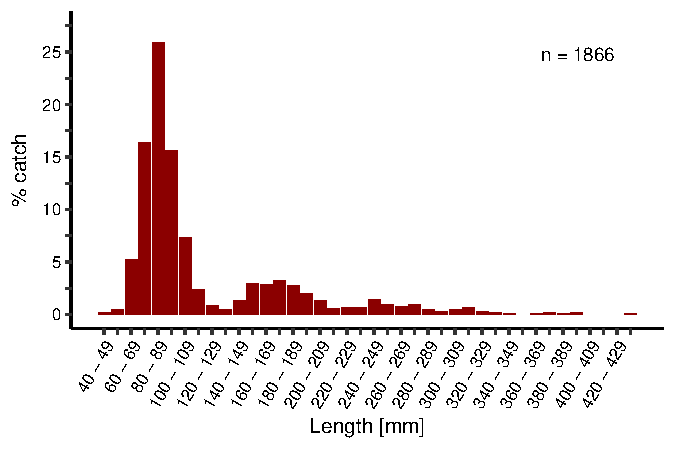
\includegraphics[width=.7\textwidth]{images/brown_single.pdf}                %% Width, Image file COLOR
	\caption{Length-frequency plot showing population structure of brown trout in the River Ois.}        %% Figure Caption
	\label{fig:brown_single}                                                       %% Figure label key
\end{figure}

Comparing the length-frequency of the two sampled sections~(\cref{fig:brown_section}) shows that the Hinterleiten has a higher portion of YOY at approximately 80\% of the total catch, while The 1+ fish accounted for only 13\% of total catch.
The YOY in the Rothschild section accounted for 60\% of total catch and the 1+ age class represented around 28\% of total catch.

\begin{figure}[!htb]                              %% Brown in section
	\center
	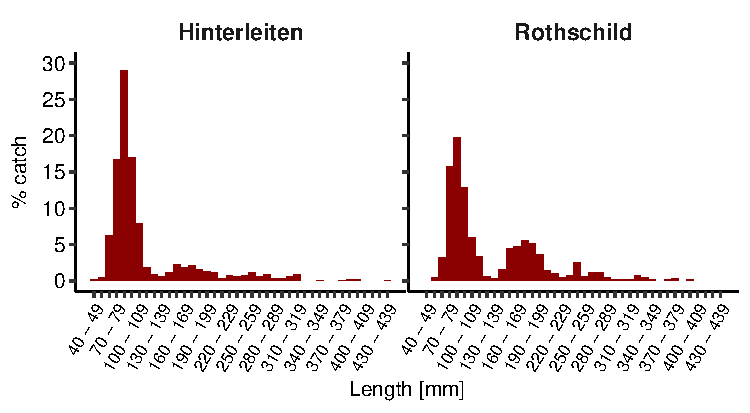
\includegraphics{images/brown_section.pdf}                %% Width, Image file COLOR
	\caption{Length-frequency plot showing the difference in population structure of brown trout in two sections of the River Ois.}   %% Figure Caption
	\label{fig:brown_section}                                                       %% Figure label key
\end{figure}

A comparison of brown trout populations in different mesohabitats can be seen in~\cref{fig:brown_meso}.
All age classes are present in the pool habitat, with YOY accounting for less than 50\% total catch.
1+ and 2+ fish accounted for 28\% and 15\% of the pools respectively.
Run mesohabitats contained more juvenile fish with YOY representing 72\% of the population.
21\% of the population were 1+ fish leaving less than 7\% fish greater than 220mm in length.
The riffles contained the highest percentage of YOY at 87\%.
1+ fish made up 11\% of the population, with very few fish larger than 220mm.

\begin{figure}[!htb]                              %% Brown in meso
	\center
	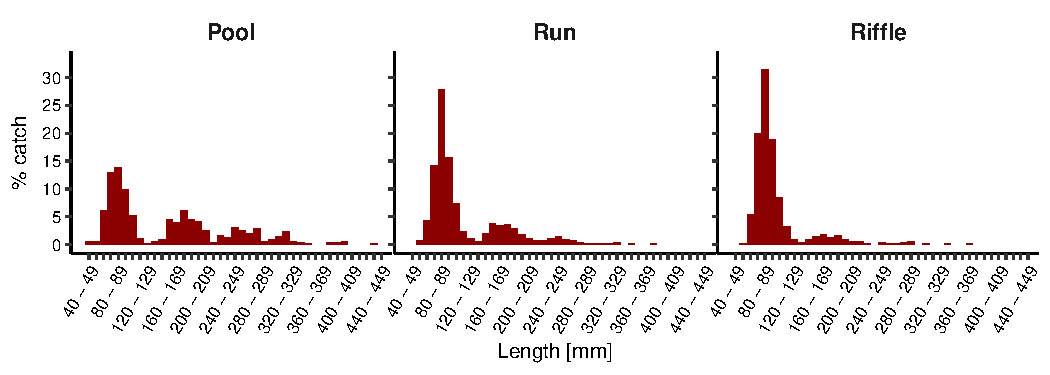
\includegraphics[width=\textwidth]{images/brown_meso}                %% Width, Image file COLOR
	\caption{Length-frequency plot of brown trout populations in different mesohabitats of River Ois.}        %% Figure Caption
	\label{fig:brown_meso}                                                       %% Figure label key
\end{figure}

A representation of the brown trout population in each of the sampled sites is shown in~\cref{fig:brown_mix}.
It can be seen that larger fish tend to occur most often in pool mesohabitats, less frequently in runs, and rarely in riffles.
YOY represent the majority of caught fish in the riffles and runs of all three sections.
The lower riffle of the Hinterleiten contained the youngest population with YOY accounting for 92\% of total catch.
All mesohabitats within the Rothschild showed a higher proportion of large fish when compared with the Hinterleiten habitats.
The Rothschild pool was unique in that YOY represented only 29\% of the catch, with 1+ fish (48\%), 2+ fish (17\%) and fish larger than 300mm (6\%) accounting for the remainder.

\begin{figure}[!htb]                              %% Brown mixed grid
	\center
	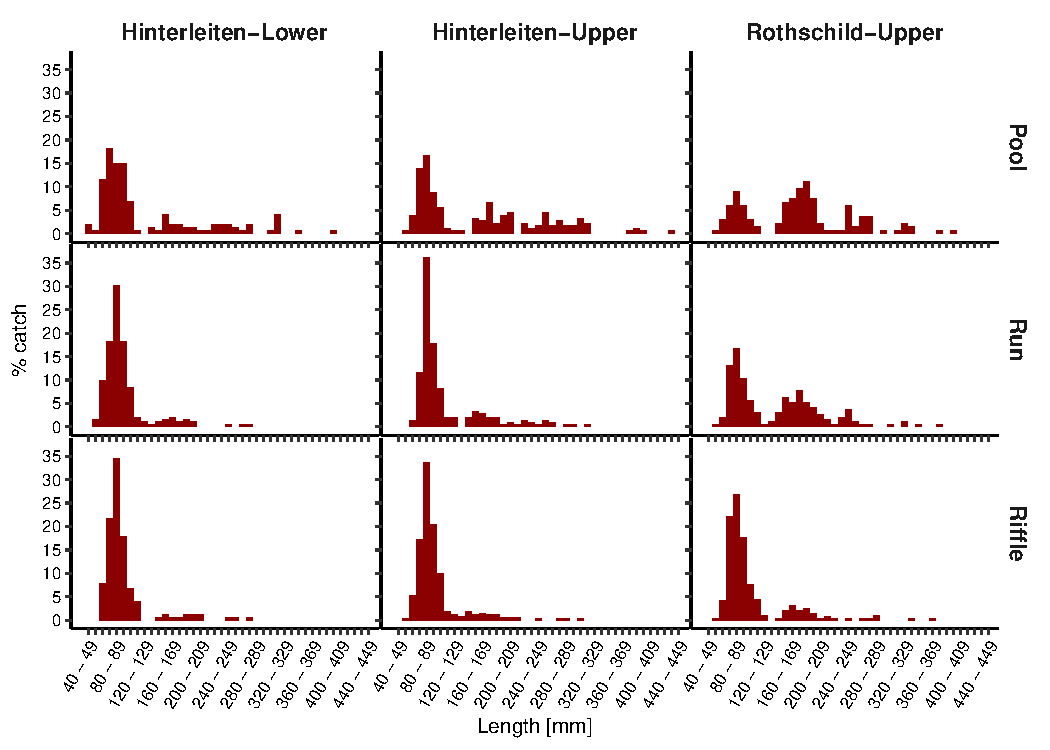
\includegraphics[width=\textwidth]{images/brown_mix}                %% Width, Image file COLOR
	\caption{Length-frequency plots of brown trout in the 9 sampled sections.}        %% Figure Caption
	\label{fig:brown_mix}                                                       %% Figure label key
\end{figure}


\paragraph{Rainbow trout (\textit{Onchorhynchus mykiss})}\label{sec:ois_rt_lf}

The population structure of rainbow trout sampled in the Ois can be seen in~\cref{fig:rain_single}.
All ages classes are present, with a high percentage of YOY fish.
Rainbow trout YOY were defined as individuals less than 150mm in length and accounted for 67\% of the 383 rainbow trout that were sampled.
1+ fish (\textgreater150mm) were 20\%, 2+ fish (\textgreater250mm) were 10\% and fish larger than 350mm were less than 3\% of the total catch.

\begin{figure}[!h]                              %% Rainbow in Ois
	\center
	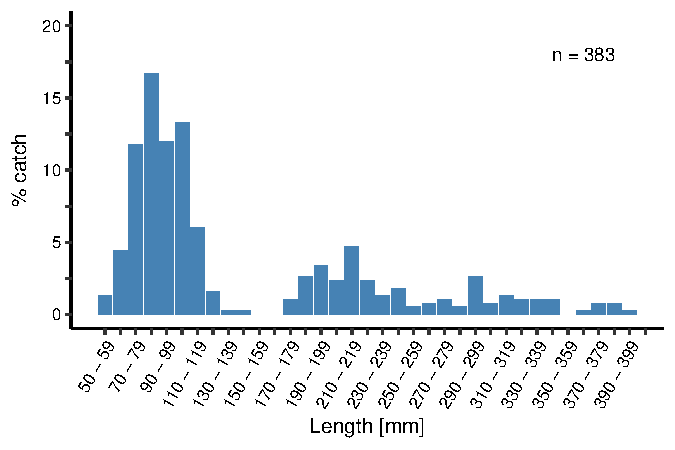
\includegraphics[width=.7\textwidth]{images/rain_single.pdf}     %% Width, Image file COLOR
	\caption{Length-frequency plot showing population structure of rainbow trout in the River Ois.}        %% Figure Caption
	\label{fig:rain_single}           %% Figure label key
\end{figure}

The rainbow trout populations between the two sections are quite similar~(\cref{fig:rain_section}) with the Rothschild having a slightly older population.
YOY had the highest portion of total catch in the Hinterleiten with 70\% and 63\% in the Rothschild.
1+ fish were comparable with 19\% and 20\%.
The share of 2+ fish was lower in the Hinterleiten (10\%) than the Rothschild (12.5\%).
350mm plus fish were mostly absent from the Hinterleiten, but contributed 6\% of the total catch in the Rothschild.

\begin{figure}[!h]                              %% Rainbow in sections
	\center
	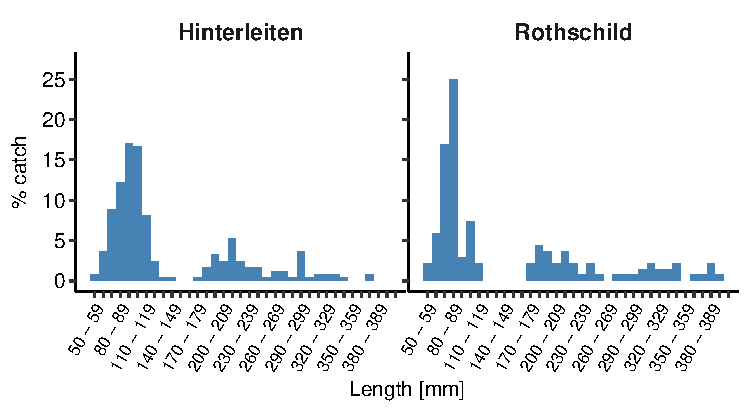
\includegraphics{images/rain_section.pdf}    %% Width, Image file COLOR
	\caption{Length-frequency plot showing the difference in population structure of rainbow trout in two sections of the River Ois.} %% Figure Caption 
	\label{fig:rain_section}     %% Figure label key
\end{figure}

The age class distribution of rainbow trout among the mesohabitats~(\cref{fig:rain_meso}) is comparable to the brown trout~(\cref{fig:brown_meso}).
The pool sections are characterized by an almost even distribution among the age classes.
The pools were composed of 38\% YOY, 31\% 1+ fish, 27\% 2+ fish and 4\% were larger than 350mm.
The runs had a younger population structure with 71\% of the total catch being YOY. 1+ fish (22\%), 2+ fish (5\%) and \textgreater350mm fish made up just over 2\% in the remainder of the runs.
Riffles had the youngest population by far, with 91\% being YOY.
The riffles also contained 7\% 1+ fish, 2\% 2+ fish and no fish larger than 350mm.

\begin{figure}[!htb]                              %% Rainbow in Meso
	\center
	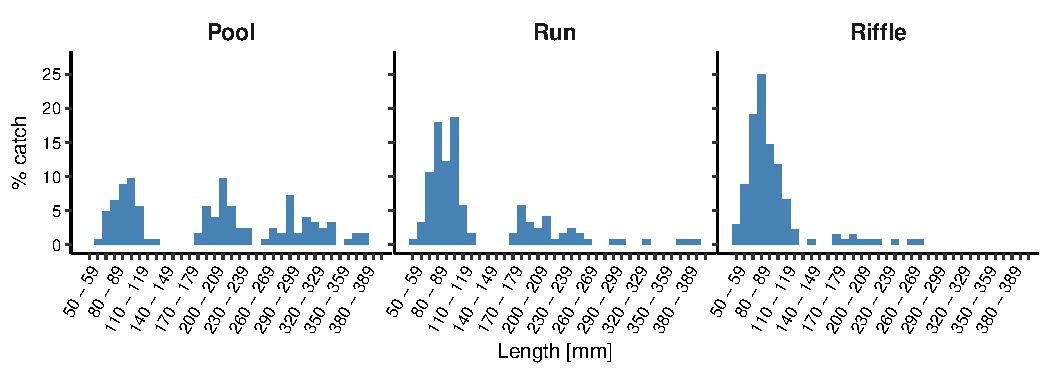
\includegraphics[width=\textwidth]{images/rain_meso.pdf}                %% Width, Image file COLOR
	\caption{Length-frequency plot of rainbow trout populations in different mesohabitats of River Ois.}        %% Figure Caption
	\label{fig:rain_meso}                                                       %% Figure label key
\end{figure}

The length-frequency of rainbow trout the sampled sections~(\cref{fig:rain_mix}) also follow the trends identifiable in the brown trout~(\cref{fig:brown_mix}).
Larger fish can be found in the pools, while more juveniles are found in runs and riffles.
Populations between the three sections are quite similar.
More detailed analysis is not possible due to the small sample size.

\begin{figure}[!htb]                              %% Rainbow in mixed grid
	\center
	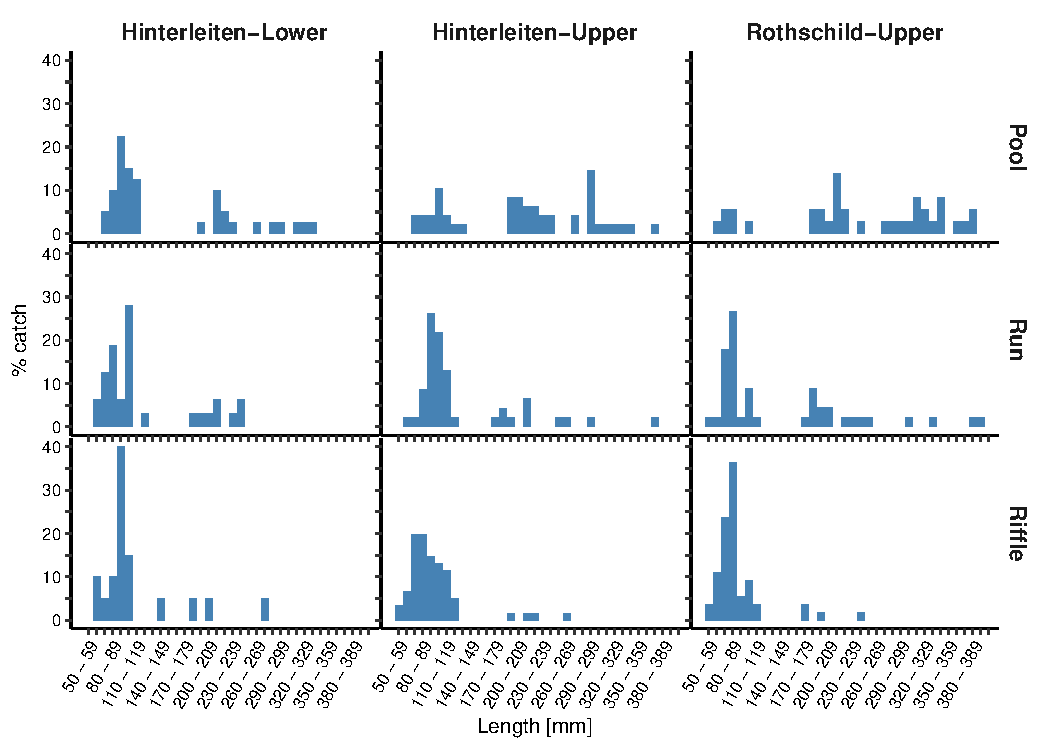
\includegraphics[width=\textwidth]{images/rain_mix.pdf}                %% Width, Image file COLOR
	\caption{Length-frequency plots of rainbow trout in the 9 sampled sections.}        %% Figure Caption
	\label{fig:rain_mix}                                                       %% Figure label key
\end{figure}


















\subsubsection{Abundance and Biomass}\label{sec:ois_ab_mass}

The sum of total catch for each sampled site was divided by the area sampling to calculate abundance and biomass.
These values were then weighted according to the habitat distribution of the Hinterleiten and Rothschild sections.
The ratio of mesohabitats can be seen in~\cref{tab:habitat_distribution}.

\begin{table}[!htb]                                 %% Habitat distribution
	\small                   
	\centering
	\caption{Habitat distribution among the river sections.}
	\begin{tabular}{ l c c }
		\toprule
		&	Hinterleiten  	&	Rothschild 	\\
		mesohabiat	&	\scriptsize[\%]	&	\scriptsize[\%]	\\
		\hline
		\hline
		pool	&	30	&	10	\\
		run     & 	27  & 	50	\\
		riffle  & 	43  & 	40	\\
		\bottomrule
	\end{tabular}
	\label{tab:habitat_distribution}%
\end{table}%

The combined abundance and biomass of all salmonid species can be seen in~\cref{fig:AB_all_species}.
The calculated abundance of the Hinterleiten was 2922 individuals per hectare.
Of those individuals, 1299 could be found in riffles, 1016 in pools, and 607 in runs.
The Rothschild had slightly less abundance at 2396 individuals per hectare.
Of these, 1065 could be found in riffles, 777 in runs, and 553 individuals in pools.
Due to habitat distribution, the Hinterleiten had a higher abundance than the Rothschild.


\begin{figure}[!htb]                              %% All species
	\center
	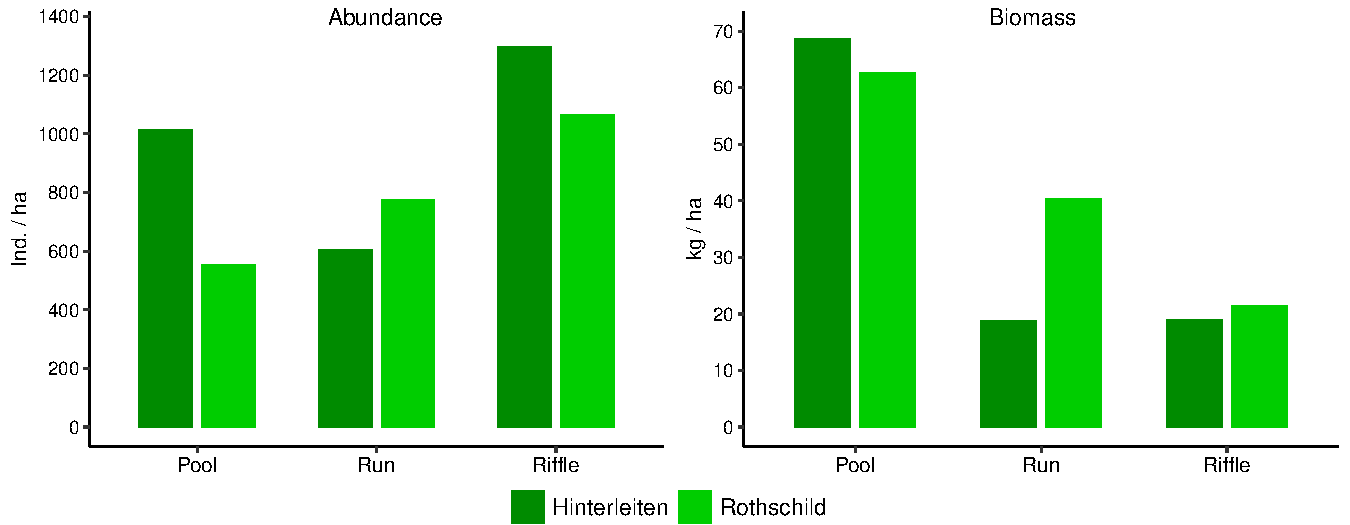
\includegraphics[width=.9\textwidth]{images/all_species.pdf}                %% Width, Image file COLOR
	\caption{Weighted distribution of combined abundance and biomass of salmonid species in the mesohabitats of two sampled sections.}        %% Figure Caption
	\label{fig:AB_all_species}                                                       %% Figure label key
\end{figure}

\begin{figure}[!htb]                              %% Brown trout
	\center
	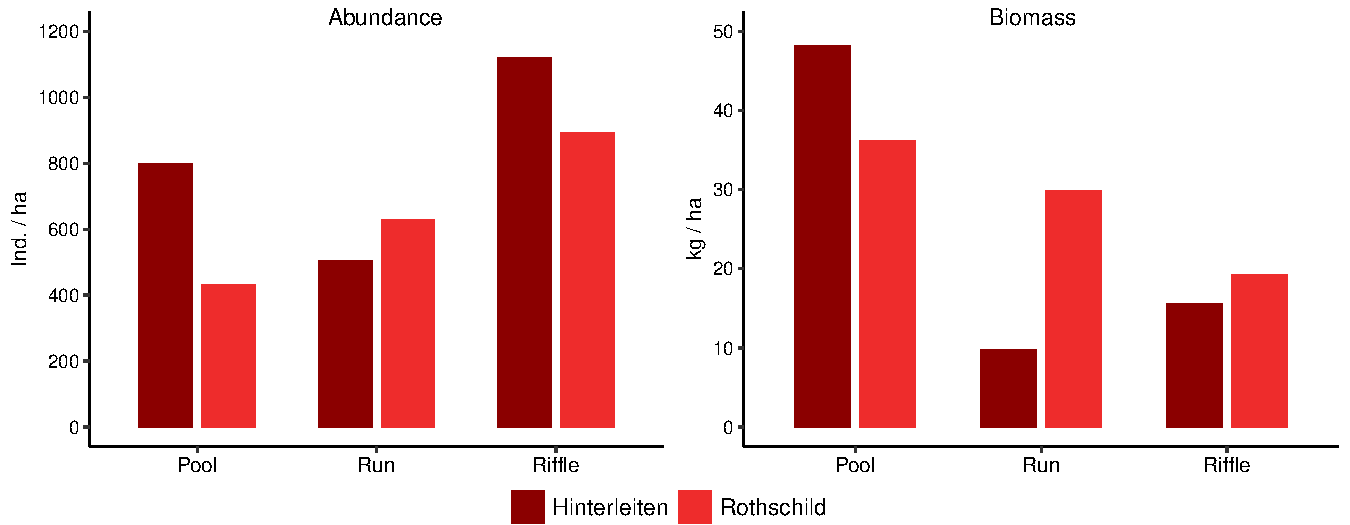
\includegraphics[width=.9\textwidth]{images/brown_trout.pdf}                %% Width, Image file COLOR
	\caption{Weighted distribution of abundance and biomass of brown trout population in the mesohabitats of two sampled sections.}        %% Figure Caption
	\label{fig:AB_brown}                                                       %% Figure label key
\end{figure}

\begin{figure}[!htb]                              %% Rainbow trout
	\center
	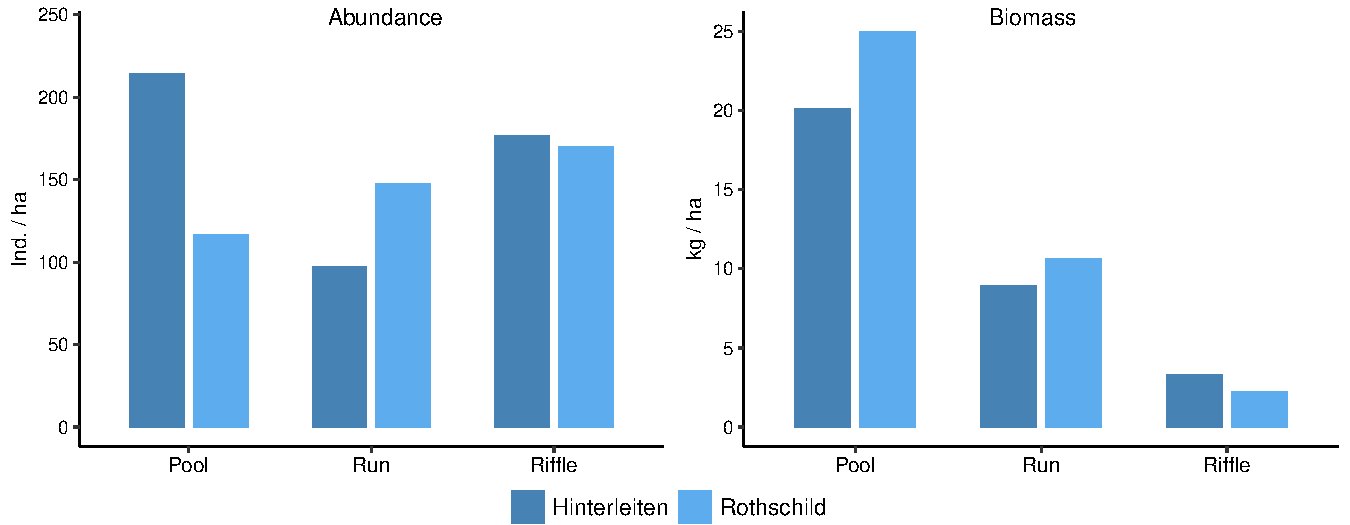
\includegraphics[width=.9\textwidth]{images/rainbow_trout.pdf}                %% Width, Image file COLOR
	\caption{Weighted distribution of abundance and biomass of rainbow trout population in the mesohabitats of two sampled sections.}        %% Figure Caption
	\label{fig:AB_rainbow}                                                       %% Figure label key
\end{figure}

%			\begin{figure}[!htb]                              %% Grayling
%				\center
%				\includegraphics[width=.9\textwidth]{images/grayling.pdf}                %% Width, Image file COLOR
%				\caption{Abundance and biomass of grayling in mesohabitats.}        %% Figure Caption
%				\label{fig:AB_gray}                                                       %% Figure label key
%			\end{figure}

\begin{figure}[!htb]                              %% All species in meso habitats
	\center
	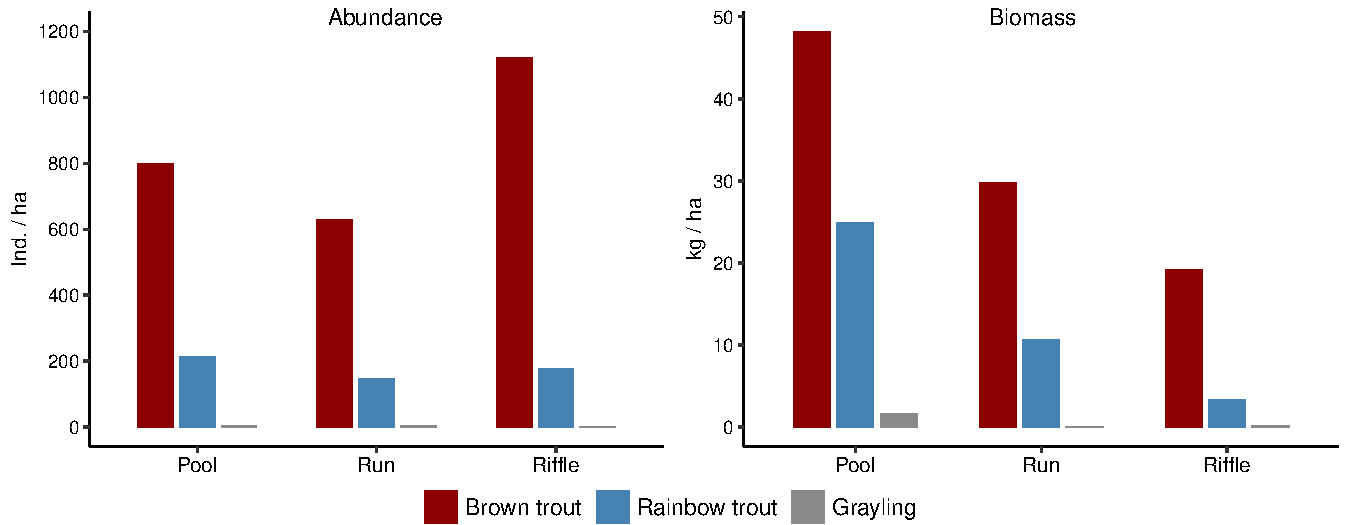
\includegraphics[width=.9\textwidth]{images/mesohabitat.pdf}                %% Width, Image file COLOR
	\caption{Comparison of the distributed abundance and biomass of salmonid species in mesohabitat components of the River Ois.}        %% Figure Caption
	\label{fig:AB_meso}                                                       %% Figure label key
\end{figure}

\begin{figure}[!htb]                              %% All species in sections
	\center
	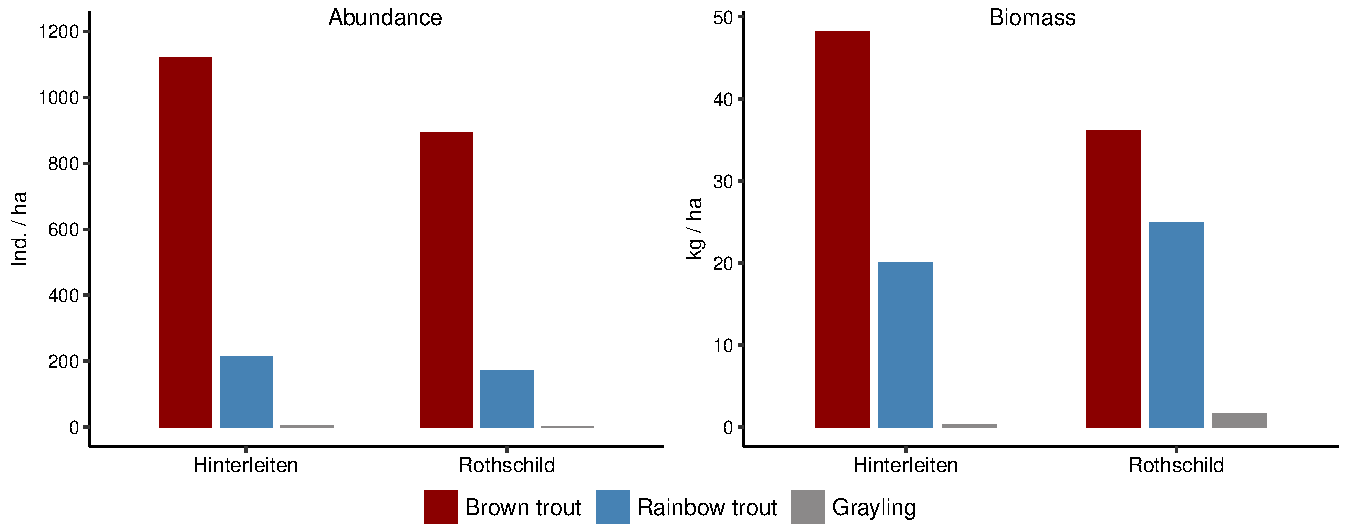
\includegraphics[width=.9\textwidth]{images/section.pdf}                %% Width, Image file COLOR
	\caption{Comparison of distributed abundance and biomass of salmonid species in Hinterleiten and Rothschild sections.}        %% Figure Caption
	\label{fig:AB_section}                                                       %% Figure label key
\end{figure}



\begin{table}[!htb]                                 %% Habitat distribution
	\small                   
	\centering
	\caption{Habitat distribution among the river sections.}
	\begin{tabular}{lllllllllll}
		\toprule
		 &  &  & Hinterleiten &  &  &  &  & Rothschild &  &  \\
		 & Habitat.dis & Ind.ha & kg.ha & Ind.ha.dis & kg.ha.dis & Habitat.dis & Ind.ha & kg.ha & Ind.ha.dis & kg.ha.dis \\
		 \hline
		 \hline
		All Species & \% &  &  &  &  & \% &  &  &  &  \\
		Pool & 30 & 3387 & 229.0 & 1016 & 68.7 & 13 & 4193 & 475.2 & 553 & 62.7 \\
		Run & 27 & 2247 & 69.5 & 607 & 18.8 & 47 & 1661 & 86.5 & 777 & 40.5 \\
		Riffle & 43 & 3022 & 44.3 & 1299 & 19.1 & 40 & 2644 & 53.3 & 1065 & 21.5 \\
		Brown trout &  &  &  &  &  &  &  &  &  &  \\
		Pool & 30 & 2661 & 160.8 & 798 & 48.3 & 13 & 3286 & 273.8 & 434 & 36.2 \\
		Run & 27 & 1874 & 36.2 & 506 & 9.8 & 47 & 1346 & 63.8 & 630 & 29.9 \\
		Riffle & 43 & 2606 & 36.2 & 1120 & 15.6 & 40 & 2213 & 47.7 & 892 & 19.2 \\
		Rainbow trout &  &  &  &  &  &  &  &  &  &  \\
		Pool & 30 & 714 & 67.0 & 214 & 20.1 & 13 & 883 & 189.2 & 117 & 25.0 \\
		Run & 27 & 360 & 33.2 & 97 & 9.0 & 47 & 315 & 22.7 & 148 & 10.6 \\
		Riffle & 43 & 411 & 7.8 & 177 & 3.3 & 40 & 423 & 5.6 & 170 & 2.3 \\
		Grayling &  &  &  &  &  &  &  &  &  &  \\
		Pool & 30 & 12 & 1.1 & 4 & 0.3 & 13 & 25 & 12.2 & 3 & 1.6 \\
		Run & 27 & 13 & 0.1 & 3 & 0.0 & 47 & 0 & 0.0 & 0 & 0.0 \\
		Riffle & 43 & 5 & 0.3 & 2 & 0.2 & 40 & 0 & 0.0 & 0 & 0.0 \\
		\bottomrule
	\end{tabular}
\end{table}

